\documentclass[tikz,border=0.1in]{standalone}
\usepackage{tikz}
\usetikzlibrary{positioning, arrows.meta, fit, backgrounds, calc}
\usepackage[T1]{fontenc}
\usepackage{amssymb}
\usepackage[scaled=0.95]{helvet}
\renewcommand{\familydefault}{\sfdefault}

\definecolor{miamired}{HTML}{C3142D}
\definecolor{agentblue}{HTML}{1D5FAD}
\definecolor{evalgold}{HTML}{EFDB72}
\definecolor{nonfund}{HTML}{CCC9B8}

\tikzset{
  gate/.style  = {rectangle, rounded corners, draw=miamired, ultra thick,
                  fill=miamired!8, align=center, text width=3.35cm, minimum height=1.65cm,
                  font=\small\bfseries, inner sep=5pt},
  work/.style  = {rectangle, rounded corners, draw=agentblue, ultra thick,
                  fill=agentblue!6, align=center, text width=3.35cm, minimum height=1.65cm,
                  font=\small\bfseries, inner sep=5pt},
  check/.style = {rectangle, rounded corners, draw=evalgold!80!black, ultra thick,
                  fill=evalgold!22, align=center, text width=3.35cm, minimum height=1.65cm,
                  font=\small\bfseries, inner sep=5pt},
  outbox/.style = {rectangle, rounded corners, draw=nonfund, ultra thick,
                  fill=nonfund!30, align=center, text width=3.35cm, minimum height=1.65cm,
                  font=\small\bfseries, inner sep=5pt},
  lab/.style   = {font=\small, align=center},
  flow/.style  = {ultra thick, -{Stealth[length=3mm]}, draw=miamired!65},
  loop/.style  = {ultra thick, -{Stealth[length=3mm]}, draw=evalgold!80!black},
  reuse/.style = {ultra thick, -{Stealth[length=3mm]}, draw=gray!60, dashed},
}

\begin{document}
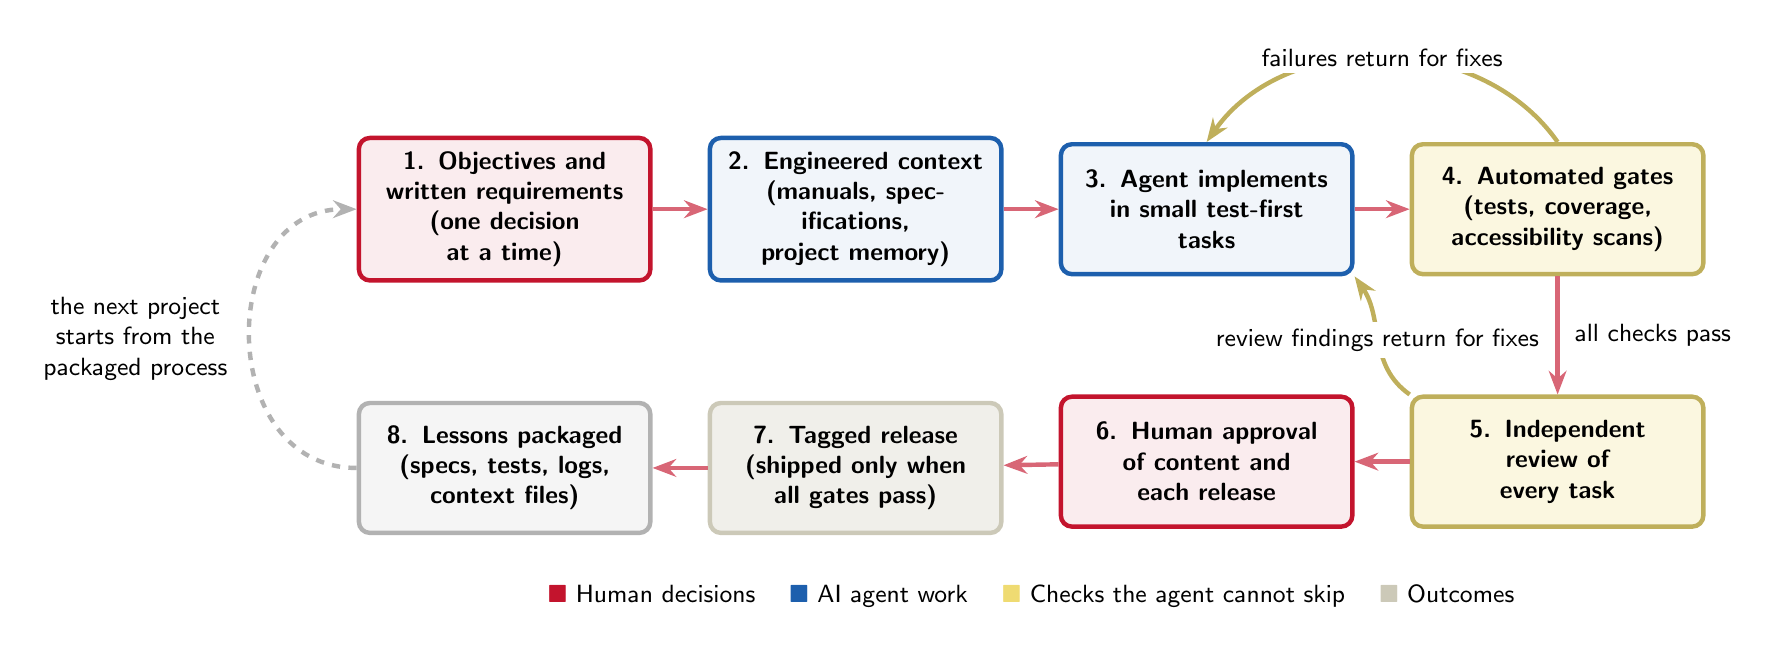
\begin{tikzpicture}[node distance=1.5cm and 0.7cm]

% Row 1, left to right: from decisions to automated checks
\node (g1) [gate]                 {1. Objectives and\\written requirements\\(one decision at a time)};
\node (w1) [work, right=of g1]    {2. Engineered context\\(manuals, specifications,\\project memory)};
\node (w2) [work, right=of w1]    {3. Agent implements\\in small test-first\\tasks};
\node (c1) [check, right=of w2]   {4. Automated gates\\(tests, coverage,\\accessibility scans)};

% Row 2, right to left: from review to packaged lessons (serpentine)
\node (c2) [check, below=of c1]   {5. Independent\\review of\\every task};
\node (g2) [gate, below=of w2]    {6. Human approval\\of content and\\each release};
\node (r1) [outbox, below=of w1]  {7. Tagged release\\(shipped only when\\all gates pass)};
\node (l1) [outbox, below=of g1, draw=gray!60, fill=gray!8] {8. Lessons packaged\\(specs, tests, logs,\\context files)};

% Main serpentine flow
\draw [flow] (g1) -- (w1);
\draw [flow] (w1) -- (w2);
\draw [flow] (w2) -- (c1);
\draw [flow] (c1) -- node[lab, right=2pt] {all checks pass} (c2);
\draw [flow] (c2) -- (g2);
\draw [flow] (g2) -- (r1);
\draw [flow] (r1) -- (l1);

% Fix loops back to construction; labels sit on their own arrows so the
% ownership is unambiguous and the line breaks around the text.
\draw [loop] (c1.north) to[out=125,in=55] node[lab, fill=white, inner sep=2.5pt] {failures return for fixes} (w2.north);
\draw [loop] (c2.north west) to[out=145,in=-55] node[lab, fill=white, inner sep=2.5pt, pos=0.5] {review findings return for fixes} (w2.south east);

% Reuse loop into the next cycle (adjacent column)
\draw [reuse] (l1.west) to[out=180,in=180, looseness=1.4] node[lab, left=2pt, text width=2.5cm] {the next project starts from the packaged process} (g1.west);

% Legend
\node [font=\small, anchor=north] at ($(g2.south)!0.5!(r1.south)+(0,-0.55)$) {%
  \textcolor{miamired}{$\blacksquare$}~Human decisions \quad
  \textcolor{agentblue}{$\blacksquare$}~AI agent work \quad
  {\color{evalgold}$\blacksquare$}~Checks the agent cannot skip \quad
  {\color{nonfund}$\blacksquare$}~Outcomes};

\end{tikzpicture}
\end{document}
